\documentclass{article}

% -------------- PACOTE GERAL -------------- %
\usepackage{helper/helper}
\usepackage[a4paper, total={6in, 8in}]{geometry}
% \usepackage[a5paper]{geometry}

% -------------- CONFIGURACOES DA BIBLIOGRAFIA -------------- %
\addbibresource{bibliografia.bib}

% -------------- TITULO E INFORMACOES -------------- %
\title{Condicionamento}
\author{pão}
\date{Julho de 2025}

% -------------- DOCUMENTO -------------- %
\begin{document}
\maketitle

% Sumario
\tableofcontents
\pagebreak

% -------------- SECOES -------------- %
\section{Introdução}
A ideia inicial é a partir de um conjunto aleatório de posições e velocidades obter um novo conjunto de posições e velocidades que tenham determinadas integrais primeiras. Nesse caso aqui, não vou mexer nas massas.

Ah, de antemão vou considerar que no sorteio já consigo o centro de massas na origem. Isso é algo que preciso pensar depois, mas vou supor que já está feito.

Não é o objetivo aqui pensar em como obter valores iniciais antes do condicionamento. Talvez caiba escrever sobre no futuro, mas por agora vou supor que já tenho todos os valores iniciais em mãos e vou apenas manipulá-los.

\subsection{O que acontece se começamos com partículas sem velocidade?}
Se o sistema começa com energia cinética nula, as partículas vão para o centro e se intereferem mutuamente, ganhando momento angular em troca de perderem velocidade radial. Após o choque inicial, o sistema perde uma considerável quantidade de partículas que conseguem energia suficiente para escaparem, e o sistema segue para a relaxação violenta. Segundo testes de Standish em 1968, cerca de 15\% das partículas escapam. Experimentos de Lecar e Cohen (1972) em 1 dimensão também confirmam que a distribuição em equilíbrio só ocorre na parte principal (centro).



\section{Problema clássico de N-corpos}
\subsection{Propriedades}

O PNCG tem algumas propriedades importantes que valem ser ressaltadas.

\subsubsection{Desigualdade de Sundman}

\begin{theorem}[Desigualdade de Sundman]
    Sejam $\vet J$ o momento angular, $I$ o momento de inércia e $E$ a energia total de um PNCG. Então $\norma{\vet J}^2 \leq I(\ddot I - 2E)$.
\end{theorem}
\begin{proof}
    Tem no TCC. É só Cauchy-Schwarz.
\end{proof}

Seu impacto se dá da seguinte forma. Considere a transformação $\tilde{\vet q} = \alpha^{-1} \vet q$ visando obter $\tilde{\vet J}$ e $\tilde E$. No caso do PNCG clássico, a Identidade de Lagrange-Jacobi nos garante que $\ddot I = 4E - 2V$, então a desigualdade de Sundman assume o formato
\begin{equation}
    \tilde c^2 \leq 2 \tilde{I} (\tilde{E} - \tilde V),
    \quad
    \tilde c = \norma{\tilde{\vet J}}.
\end{equation}
Observe que $I$ é uma função homogênea de grau 2, e como $V$ é homogêneo de grau -1, temos:
\begin{equation}
    \tilde c^2 \leq 2 \alpha^{-2} I_0 (\tilde E - |\alpha| V_0) = 2 \alpha^{-2} I_0 \tilde E - 2 \dfrac{|\alpha|}{\alpha^2} I_0 V_0.
\end{equation}
Podemos multiplicar ambos os lados por $\alpha^2 > 0$:
\begin{equation}\label{eq:inequacao_sundman}
    \tilde c^2 \alpha^2 - 2 I_0 \tilde E + 2 |\alpha| I_0 V_0 \leq 0.
\end{equation}

Independente do sinal de $\alpha$, o que temos é uma inequação de segundo grau para $\alpha$ com coeficiente de segundo grau positivo, o que significa que só existe solução se a equação tiver alguma solução. O discriminante é:
\begin{equation}\label{eq:delta_sundman}
    \Delta_{Sundman} = 4 I_0^2 V_0^2 + 8 \tilde c^2 I_0 \tilde E,
\end{equation}
e uma solução existe se, e somente se,
\begin{equation}
    I_0 V_0^2 \geq -2 \tilde c^2 \tilde E.
\end{equation}
A restrição imposta por $\Delta_{Sundman}$ de fato não importa se $\tilde E \geq 0$. Mas caso contrário, identifica se a energia total é suficiente para atender a quantidade de rotação exigida através de $\tilde c^2$.

% Preciso escolher um nome melhor para isso
\subsubsection{Desigualdade da inércia}
Seja $\bm W_T = - \bm I_T$, para facilitar a notação. Sabemos que matriz $\bm W_T$ é real e simétrica, e na suposição de que os corpos não sejam colineares (!!!) a matriz é também positiva definida (portanto SPD). Uma matriz com essas propriedades é invertível, e tanto ela quanto sua inversa definem produtos internos e consequentemente normas [ADICIONAR REFERENCIAS DISSO]. Dessa forma, podemos escrever que:
\begin{equation}
    \vet u^T \bm W_T^{-1} \vet u = \prodint{\vet u}{\vet u}_{\bm W_T^{-1}}.
\end{equation}
Pela equivalência de normas, temos que:
\begin{equation}\label{eq:equivalencia_normas_W}
    \lambda_{min} (\bm W_T^{-1}) \leq \dfrac{\vet u^T \bm W_T^{-1} \vet u}{\vet u^T \vet u} \leq \lambda_{max} (\bm W_T^{-1}),
\end{equation}
onde os extremos são o menor e o maior autovalor de de $\bm W_T^{-1}$, respectivamente. Por ser SPD, seus autovalores são todos reais positivos e, mais ainda, $\lambda_i (\bm W_T^{-1}) = 1/\lambda_i(\bm W_T)$. Vale observar também que o momento de inércia pode ser escrito em função dos autovalores de $\bm W_T$:
\begin{equation}\label{eq:momento_inercia_autovalores_W}
    I = \dfrac{1}{2} tr \bm W_T = \dfrac{1}{2} \sum_{i=1}^3 \lambda_i (\bm W_T) \geq \dfrac{1}{2} \lambda_{max}(\bm W_T).
\end{equation}
Aplicando (\ref{eq:momento_inercia_autovalores_W}) em (\ref{eq:equivalencia_normas_W}) conseguimos o seguinte:
\begin{equation}\label{eq:desigualdade_inercia}
    \dfrac{1}{2I} \leq \lambda_{min} (\bm W_T^{-1}) \leq \dfrac{\vet u^T \bm W_T^{-1} \vet u}{\vet u^T \vet u}
    \Rightarrow
    2 \vet u^T \bm W_T^{-1} \vet u \geq \vet u^T \vet u I^{-1}.
\end{equation}

Essa desigualdade é particularmente interessante quando estamos trabalhando com vetores ligados ao PNCG. Pensando no momento angular $\vet J$, por exemplo, $\vet J^T \bm W_T^{-1} \vet J$ está relacionado com o movimento angular do sistema, e podemos relacioná-lo com sua própria norma:
\begin{equation}\label{eq:desigualdade_inercia_angular}
    2 \vet J^T \bm W_T^{-1} \vet J \geq || \vet J ||^2 I^{-1}.
\end{equation}

\subsection{Pensando separadamente}
O problema clássico tem o potencial
\begin{equation}
    V(\vet q) = - G \sum_{a < b} \dfrac{m_a m_b}{r_{ab}},
\end{equation}
que é uma função homogênea com grau -1, ou seja, sendo $k \in \R$, temos
\begin{equation}
    V(k \vet q) = |k|^{-1} V(\vet q).
\end{equation}
Também vale observar que a energia cinética $T$ é uma função homogênea de grau 2, pois $T(k \vet p) = k^2 T(\vet p)$. Com isso, se quisermos obter uma determinada energia $\tilde E$, podemos buscar $\tilde{\vet q_a} = \alpha^{-1} \vet q_a$ e $\tilde{\vet p_a} = \beta \vet p_a$ de modo que
\begin{equation}
    T(\tilde{\vet p_a}) + V(\tilde{\vet q}) = \beta^2 T_0 + \alpha V_0 = \tilde E.
\end{equation}

Existem muitas formas de lidar com isso, sendo possível obter qualquer $\tilde E \geq 0$ apenas com $\beta$. No geral, podemos tomar, por exemplo,
\begin{equation}
    \alpha = 1 + \dfrac{\tilde E}{V_0},
    \quad
    \beta = \sqrt{-\dfrac{V_0}{T_0}}.
\end{equation}
Essa forma tem alguma vantagem? Não sei.

Já para o momento linear total, se queremos obter $\tilde P \in \R^3$ precisamos aplicar um tipo de "translação" nas velocidades, semelhante ao que pode ser feito para anular o centro de massas. Precisamos encontrar um vetor $\vet w_{\tilde P}$ tal que, definindo $\tilde{\vet p_a} = \vet p + m_a \vet w_{\tilde P}$, consigamos:
\begin{align}\label{eq:transformacao_momento_linear}
    \sum_{a=1}^N \tilde{\vet p_a} = \vet P_0 + M \vet w_{\tilde{\vet P}} = \tilde{\vet P} \
    \Rightarrow \ \vet w_{\tilde{\vet P}} = M^{-1} (\tilde{\vet P} - \vet P_0)
\end{align}

Para o momento angular, desenvolvemos independentemente uma forma de transformá-lo, mas que já constava em \cite[p.135]{aarseth_gravitational_2003} para um caso específico de 2 corpos.

De toda forma, existem diferenças na forma de tratar conforme a dimensão do problema. Se temos um conjunto de dados planar, o momento angular pode ser visto como um escalar, uma vez que $\vet J = (0, 0, J)$, então podemos buscar $\vet \omega = (0, 0, \omega)$ e definir $\tilde{\vet p_a} = \vet p_a + m_a \vet q_a \times \vet \omega$. Temos:
\begin{equation}
    \sum_{a=1}^N \vet q_a \times \tilde{\vet p_a}
    = \vet J_0 + \sum_{a=1}^N m_a \vet q_a \times (\vet q_a \times \vet \omega).
\end{equation}
Nesse caso bidimensional, $\vet q_a \times \vet \omega = \omega (-\vet q_a^{(2)}, \vet q_a^{(1)}, 0)$, e logo $\vet q_a \times (\vet q_a \times \vet \omega) = \vet \omega \norma{\vet q_a}^2$. Impondo a restrição:
\begin{equation}
    \vet \omega = \dfrac{1}{I_0}(\tilde{\vet J} - \vet J_0).
\end{equation}

\begin{figure}[H]
    \centering
    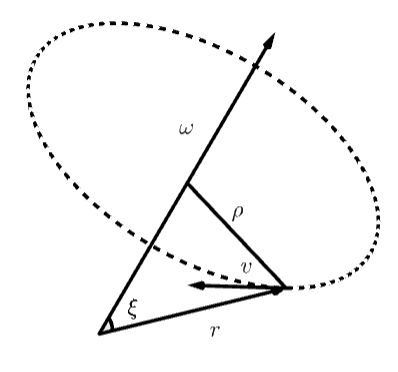
\includegraphics[width=0.3\linewidth]{img/rotacao.png}
    \caption{Representação de uma partícula e seu eixo de rotação.}
    \label{fig:angular_3d}
\end{figure}

No caso tridimensional a coisa é um pouco mais complicada. Considere uma partícula com posição $\vet r$ e um vetor $\vet \omega$ que define um eixo de rotação do qual $\vet r$ se distancia em $\rho$ e forma um ângulo $\xi$ e também cuja velocidade da partícula em relação a é $\vet v$, como na figura \ref{fig:angular_3d}. Nessa situação, temos que $\norma{\vet v} = \rho \norma{\vet \omega}$ e $\sin \xi = \rho / \norma{\vet r}$. Uma vez que $\vet v \perp \vet \omega$ e $\vet v \perp \vet v$, podemos concluir que $\vet v || \vet r \times \vet \omega$. Mais ainda, temos que:
\begin{equation}\label{eq:angular_def_omega}
    \norma{\vet r \times \vet \omega}
    = \norma{\vet r} \norma{\vet \omega} \sin \xi = \norma{\vet v}
    \Rightarrow
    \vet v = \vet r \times \vet \omega.
\end{equation}

O momento angular $\vet J$ também é um vetor perpendicular a $\vet r$ e a $\vet v$, mas $\vet J$ e $\vet \omega$ só são colineares quando $\vet r \perp \vet \omega$ (como no caso 2d). Apesar disso, a partir de (\ref{eq:angular_def_omega}) podemos construir um operador $\bm I: \R^3 \to \R^3$ em função de $m$ e $\vet r$ que leva $\vet \omega$ em $\vet J$. O operador tem a seguinte forma:
\begin{equation}
    \bm I = m
    \begin{bmatrix}
        - (r_2^2 + r_3^2) & r_1 r_2 & r_1 r_3 \\
        r_1 r_2 & - (r_1^2 + r_3^2) & r_2 r_3 \\
        r_1 r_3 & r_2 r_3 & - (r_1^2 + r_2^2)
    \end{bmatrix}.
\end{equation}
O operador $\bm I$ é denominado \textbf{tensor de inércia}, e muitas vezes aparece com o sinal oposto. Para facilitar, a partir daqui tomaremos $\bm W := \bm I$ sempre que um tensor de inércia for mencionado.

No caso de diversos corpos, a ideia é definir um eixo de rotação comum e a partir dele aplicar transformações sobre a velocidade angular de cada corpo. Seja $\bm I_T = \sum_{a=1}^N \vet q_a$ (ou seja, baseado somente nos valores pré-condicionamento). Para obter um momento angular desejado $\tilde{\vet J}$, basta encontrar um eixo $\vet \omega$ tal que $\bm I_T \vet \omega = \tilde{\vet J} - \vet J_0$ e aplicar a transformação 
\begin{equation}\label{eq:transformacao_momento_angular_3d}
    \tilde{\vet p_a} = \vet p_a + m_a \vet q_a \times \vet \omega.
\end{equation}

Diante do exposto, é evidente que as transformações propostas se sobrepõem. Por exemplo, no condicionamento da energia com $\tilde{\vet q} = \alpha^{-1} \vet q$ e $\tilde{\vet p} = \beta \vet p$, temos:
\begin{equation}
    \vet P(\tilde{\vet p}) = \beta \vet P_0,
    \quad
    \vet J(\tilde{\vet q}, \tilde{\vet p}) = \dfrac{\beta}{\alpha} \vet J_0.
\end{equation}

Além disso, qualquer "translação" nos momentos lineares, como feito em (\ref{eq:transformacao_momento_linear}) e (\ref{eq:transformacao_momento_angular_3d}), afeta fortemente a energia cinética do sistema, o que deve ser levado em conta na hora de condicionar um sistema por completo.

\subsection{Método iterativo}
Apesar da sobreposição das transformações, nas situações em que é possível obter uma tripla $(\tilde E, \tilde{\vet J}, \tilde{\vet P})$, aplicar as transformações iterativamente é um método convergente.

[SERÁ MESMO? COMO POSSO MOSTRAR ISSO?]
\subsection{Método direto}
Há, no entanto, uma forma de unir todas as transformações adequadamente. De fato, basta tomar
\begin{align}
    \tilde{\vet q_a} &= \alpha^{-1} \vet q_a, \\
    \tilde{\vet p_a} &= \beta\left(\vet p_a - \dfrac{m_a}{M} \left(\vet P - \beta^{-1} \tilde{\vet P}\right) - m_a \vet q_a \times \vet \omega\right), \\
    \bm I_T \vet \omega &= \vet J - \alpha \beta^{-1} \tilde{\vet J}.
\end{align}

Como $\alpha$ impacta fortemente no valor de $\beta$, vamos obter $\beta$ primeiro. Veja que temos o seguinte para a energia total:
\begin{equation}\label{eq:t_til_e_til_v0}
    T(\tilde{\vet p}) = \tilde E - \alpha V_0.
\end{equation}
Vamos expandir $T(\tilde{\vet p})$:
\begin{align*}
    T(\tilde{\vet p}) 
    &= \sum_{a=1}^{N} \dfrac{\beta^2}{2m_a} \norma{\vet p_a - \dfrac{m_a}{M}\left(\vet P - \beta^{-1} \tilde{\vet P}\right) - m_a \vet q_a \times \bm I_{T}^{-1} (\vet J - \alpha \beta^{-1} \tilde{\vet J})}^2.
\end{align*}
Podemos separar $\tilde T$ da seguinte forma:
\begin{equation}\label{eq:separacao_t_til}
    \tilde T = \beta^2 S_1 + S_2,
\end{equation}
onde:
\begin{align*}
    S_1 &= \sum_{a=1}^N \dfrac{1}{2m_a} \norma{\vet K_1^a}^2
    = \sum_{a=1}^N \dfrac{1}{2m_a} \norma{\vet p_a - \dfrac{m_a}{M} \vet P - m_a \vet q_a \times (\bm I_T^{-1} \vet J)}^2, \\
    S_2 &= \sum_{a=1}^N \dfrac{1}{2m_a} \norma{\vet K_2^a}^2 = \sum_{a=1}^N \dfrac{1}{2 m_a} \norma{\dfrac{m_a}{M} \tilde{\vet P} + \alpha m_a \vet q_a \times (\bm I_T^{-1} \tilde{\vet J})}^2,
\end{align*}
e não é difícil ver que $\sum_{a=1}^N m_a^{-1} \prodint{\vet K_1^a}{\vet K_2^a} = 0$.

De fato, podemos melhorar bastante as expressões de $S_1$ e $S_2$. Com algumas contas chegamos no seguinte para $S_1$:
\begin{equation}
    S_1 = T_0 - \dfrac{\norma{\vet P_0}^2}{2 M} + \dfrac{1}{2} \sum_{a=1}^N m_a \norma{\vet q_a \times \vet \omega_0}^2 + \prodint{\vet J_0}{\bm I_T^{-1} \vet J_0}.
\end{equation}
A expressão que ainda possui um somatório pode ser melhorada:
$$
\norma{\vet q_a \times \vet \omega}^2 = \norma{\vet q_a}^2 \norma{\vet \omega}^2 - \prodint{\vet q_a}{\vet \omega}^2
=
\vet \omega^T (\norma{\vet q_a}^2 Id_3 - \vet q_a \vet q_a^T) \vet \omega.
$$

Observe também que o tensor de inércia $\bm I_a$ do corpo $a$ pode ser escrito como:
$$
\bm I_a = m_a (\vet q_a \vet q_a^T - \norma{\vet q_a}^2 Id_3),
$$
então temos para a soma:
$$
\sum_{a=1}^N m_a \norma{\vet q_a \times \vet \omega_0}^2
= - \vet \omega_0^T \sum_{a=1}^N \bm I_a \vet \omega_0
= - \vet \omega_0^T \bm I_T \vet \omega_0.
$$
Como $\vet \omega_0 = \bm I_T^{-1} \vet J_0$, temos
$$
= - \vet J_0^T (\bm I_T^{-1})^T \bm I_T \bm I_T^{-1} \vet J_0
= - \vet J_0^T (\bm I_T^{-1})^T \vet J_0.
$$
Assim, $S_1$ pode ser escrito como:
\begin{equation}\label{eq:S_1}
    S_1 = T_0 - \dfrac{\norma{\vet P_0}^2}{2 M} + \dfrac{1}{2} \prodint{\vet J_0}{\bm I_T^{-1} \vet J_0}.
\end{equation}

Através da mesma propriedade é fácil ver também que:
\begin{equation}\label{eq:S_2}
    S_2 = \dfrac{||\tilde{\vet P}||^2}{2M} - \dfrac{\alpha^2}{2} \prodint{\tilde{\vet J}}{\bm I_T^{-1} \tilde{\vet J}} = \dfrac{||\tilde{\vet P}||^2}{2M} + \dfrac{\alpha^2}{2} \tilde{\sigma}.
\end{equation}

Voltando às constantes, $\beta$ fica determinado uma vez que escolhemos $\alpha$. Porém, $\alpha$ não pode ser qualquer um. Juntando as equações (\ref{eq:t_til_e_til_v0}) e (\ref{eq:separacao_t_til}) temos:
\begin{equation}\label{eq:beta1}
    \beta^2 = \dfrac{\tilde E - \alpha V_0 - S_2}{S_1}.
\end{equation}
Como $S_1, S_2, - V_0 > 0$, precisamos escolher $\alpha$ de acordo com $\tilde E$ de modo a garantir que exista tal $\beta \in \R$. Para isso, basta que $\tilde E - \alpha V_0 - S_2 > 0$. Expandindo:
\begin{equation}\label{eq:inequacao_delta1}
    -\tilde E + \alpha V_0 + \dfrac{||\tilde{\vet P}||^2}{2M} + \dfrac{\alpha^2}{2} \tilde \sigma < 0,
\end{equation}
o que novamente é uma inequação de segundo grau para $\alpha$ com coeficiente quadrático positivo, então a solução, se houver, será o intervalo aberto entre as duas raízes da equação. Como na desigualdade de Sundman, aqui o discriminante nos impõe uma condição:
\begin{equation}
    \Delta_1 = V_0^2 - \tilde \sigma (M^{-1} ||\tilde{\vet P}||^2 - 2 \tilde E) \geq 0
\end{equation}
\begin{equation}\label{eq:restricao_delta1}
    \Rightarrow
    V_0^2 \geq \tilde{\sigma} (M^{-1} ||\tilde{\vet P}||^2 - 2 \tilde E).
\end{equation}

Aqui, $\tilde \sigma M^{-1} ||\tilde{\vet P}||^2 \geq 0$, mas a existência de $\alpha$ e $\beta$ depende de $V_0^2$ vencer a energia total desejada. Vale também ressaltar que o tensor de inércia total é também homogêneo de grau 2, então não adianta tentar reescalar as posições iniciais sorteadas por algum fator, como no outro caso. \textcolor{red}{É realmente necessário aplicar alguma mudança mais profunda, mas não sei ainda se ela sequer existe. Um caminho possível a partir daqui é analisar algo como a esperança sobre $V_0$ e $I_0$ a partir da distribuição e tal, e ai ter algo estatístico para falar: "olha, muito provavelmente não vai dar certo, escolha valores diferentes".}

De fato, a restrição do $\Delta_1$ é uma malha mais fina que a restrição de Sundman. Pela equação (\ref{eq:desigualdade_inercia_angular}) sabemos que $\tilde \sigma \geq \tilde c^2 I_0^{-1}$. Retomando a condição do $\Delta_1$ em (\ref{eq:restricao_delta1}), podemos aplicar esta desigualdade:
\begin{equation}\label{eq:desigualdade_generalizada}
    V_0^2 \geq \tilde \sigma (M^{-1} ||\tilde{\vet P}||^2 - 2 \tilde E)
    \geq \tilde c^2 I_0^{-1} M^{-1} ||\tilde{\vet P}||^2 - 2 \tilde E \tilde c^2 I_0^{-1}.
\end{equation}
Observe que o obtido aqui à direita é exatamente a condição de Sundman (\ref{eq:inequacao_sundman}) com um acréscimo do momento linear total desejado. A restrição $\Delta_1$, então é uma restrição mais forte que a de Sundman e deve ser levada em conta no condicionamento de valores iniciais.
 
\subsubsection{Momentos angular e linear totais nulos}\label{subsubsection:j_p_nulos}
Nesse caso, a coisa toda só depende do sinal de $\tilde E$, pois a expressão para $\beta$ fica:
\begin{equation}
    \beta^2 = \dfrac{\tilde E - \alpha V_0}{S_1}
    \Rightarrow
    \tilde E > \alpha V_0 \Rightarrow \alpha > \tilde E / V_0.
\end{equation}

Aqui, como em todo caso, existe um sem número de possibilidades de escolhas de $\alpha$ que dependem unicamente do propósito com a simulação. Podemos escolher, por exemplo,
\begin{equation}
    \alpha = 1 + \delta(\tilde E < 0) \tilde E / V_0.
\end{equation}
Uso isso no programa porque fica fácil de generalizar para o caso com momento linear. Uma outra escolha mais complicada seria por exemplo, tomando $s_{\tilde E} = sign(\tilde E)$, para $\tilde E \neq 0$ tomar
\begin{equation}
    \alpha = \dfrac{\tilde E}{V_0} (1 - k s_{\tilde E}),
    \quad
    \beta^2 = \dfrac{\tilde E - \tilde E (1 - k s_{\tilde E})}{S_1} = \dfrac{k s_{\tilde E} \tilde E}{S_1},
\end{equation}
e se $\tilde E = 0$ não mexer nas soluções:
\begin{equation}
    \alpha = 1, \quad \beta^2 = \dfrac{- V_0}{S_1}.
\end{equation}

Mais para frente vou fazer uma análise do impacto das escolhas nos resultados.


\subsubsection{Garantindo as outras integrais primeiras}
Para garantir as outras integrais primeiras, precisamos garantir que a restrição generalizada (\ref{eq:desigualdade_generalizada}) seja satisfeita.

Se o momento linear total desejado é nulo, é fácil ver que se $\tilde E \geq 0$ ou se $||\tilde{\vet J}|| = 0$, a condição é satisfeita de imediato, então não é necessário se preocupar. Em outros casos, basta verificar se a restrição generalizada está atendida.

Se o momento angular total desejado não for nulo e a restrição for atendida, podemos tomar como $\alpha$ o ponto que é mínimo para a parábola da inequação generalizada:
\begin{equation}
    \alpha^* = - \dfrac{V_0}{\tilde \sigma}.
\end{equation}
É verdade que qualquer $\alpha^*$ tomado entre as raízes da equação de restrição funcionará, então cabe estudar como cada uma impacta no problema. De repente no equilíbrio ou coisa assim, vamos ver.

Se por outro lado quisermos $||\tilde{\vet J}|| = 0$ mas $||\tilde{\vet P}|| \neq 0$, então podemos usar (\ref{eq:inequacao_delta1}) para obter valor de $\alpha^*$:
\begin{equation}
    \alpha > -\dfrac{||\tilde{\vet P}||^2}{2M V_0} - \tilde E / V_0.
\end{equation}
No caso, como o problema aqui pode aparecer devido ao segundo termo poder ser negativo de $\tilde E < 0$, então podemos novamente buscar $\alpha$ tal que $\tilde E - \alpha V_0 - S_2 > 0$, o que fornece:
\begin{equation}
    \alpha > -\dfrac{\tilde E}{V_0} - \dfrac{||\tilde{\vet P}||^2}{2 M V_0}.
\end{equation}
Seguindo a mesma ideia da primeira sugestão para quando os momentos totais são nulos, podemos tomar:
\begin{equation}
    \alpha^* = 1 + \delta(\tilde E < 0) \dfrac{\tilde E}{V_0} - \dfrac{||\tilde{\vet P}||^2}{2 M V_0}.
\end{equation}
\subsection{Valores iniciais em equilíbrio}
Um caso particular de valores iniciais que são convenientes no que estamos estudando são valores iniciais em equilíbrio (virial), especificamente sob as condições padrão \cite{heggie_mathieu_unidades}:
\begin{equation}\label{eq:virial_condicoes_padrao_homogeneo}
    G = 1,
    \quad
    M = 1,
    \quad
    E = -\dfrac{1}{4},
    \quad
    R_V = 1.
\end{equation}
Aqui, $R_V$ é chamado \textbf{Raio de Virial} e é dado por:
\begin{equation}
    R_V \approx - \dfrac{G M^2}{2 V},
\end{equation}
o que nesse caso nos fornece $V = - 1/2$.

\begin{definition}[Equilíbrio (virial)]
    Dizemos que um sistema está em equilíbrio se $<\ddot I>_t = 0$.
\end{definition}

Lembrando da Identidade de Lagrange-Jacobi, sabemos que $\ddot I = 4 E - 2 V$, então um sistema só pode estar em equilíbrio se a média de $2 E - V$ for (aproximadamente) zero, então $E$ precisa ser negativo. Observe que as condições (\ref{eq:virial_condicoes_padrao_homogeneo}) garantem que o problema começa em equilíbrio.

Um sistema em equilíbrio pode ter um momento linear total não nulo. Nesse caso, o centro de massas não irá permanecer na origem, então não podemos omiti-lo do cálculo de $I$:
\begin{equation}
    I = \sum_{a=1}^N m_a \norma{\vet q_a - \vet q_{cm}}^2.
\end{equation}
Também é permitido ter momento angular total não nulo. Com uma energia negativa, porém, é necessário garantir que seja satisfeita a condição generalizada, uma vez que o sistema pode não ter energia suficiente para garantir rotações ou a translação do centro de massas.

Vamos considerar dois casos diferentes aqui: no primeiro, os momentos totais são nulos; no segundo, estamos interessados em condicioná-los para serem outra coisa, dentro do possível. Em ambos, a energia total é $-1/4$ e queremos que o potencial seja $-1/2$.

\subsubsection{Momentos totais nulos (Aarseth)}
Neste caso, vamos considerar um misto do apresentado até então com um algoritmo proposto por Aarseth \cite[p. 111]{aarseth_gravitational_2003}. Primeiro, supondo que já temos valores para condicionamento, precisamos normalizar as massas para obter $M=1$; para evitar extremos, procure ter $\bar m = 1/N$.

Com isso em mãos, aplicamos o método direto para obter a tripla $(-1/4, \vet 0, \vet 0)$. Isso nos deixa relativamente perto do desejado, e com os momentos nulos qualquer redimensionamento sobre as energias não terá impacto no resultado final.

Calculamos agora, pós-condicionamento inicial, $V_0$ e $T_0$, e definimos $Q_V = \sqrt{-\frac{V_0}{2T_0}}$. Tomamos então $\beta = \frac{V_0}{2 * (-1/4)} = - 2 V_0$, e aplicamos as transformações:
\begin{equation}
    \tilde{\vet q_a} = \beta \vet q_a,
    \quad
    \tilde{\vet p_a} = \dfrac{Q_V}{\sqrt \beta} \vet p_a.
\end{equation}

De fato, atingimos o que queríamos:
\begin{align}
    T(\tilde{\vet p}) &= \dfrac{Q_V^2}{\beta} T_0 
    = \dfrac{-\frac{V_0}{2 T_0}}{- 2 V_0} T_0 = 1/4, \\
    V(\tilde{\vet q}) &= \dfrac{1}{\beta} V_0
    = -\dfrac{1}{2}, \\
    E(\tilde{\vet q}, \tilde{\vet p}) &= -1/4.
\end{align}

Nessas unidades, o "mean square equilibrium velocity" é $\sigma^2 = 1/2$, então temos um crossing time constante
\begin{equation}
    t_{cr} = \dfrac{2 R_V}{\sigma} = \dfrac{2}{\sqrt 2}.
\end{equation}

\section{Problema de N-corpos amortecido}
O problema clássico de N-corpos tem uma questão numérica importante: apesar das colisões reais serem raras, corpos que passam muito próximos desestabilizam numericamente o sistema, uma vez que dividimos o potencial por um número que pode ser muito grande. Existem muitas formas de lidar com isso, e uma das mais simples é adicionar um pequeno $\varepsilon > 0$ no denominador:
\begin{equation}
    V_\varepsilon(\vet q) := - G \sum{a < b} \dfrac{m_a m_b}{\sqrt{r_{ab}^2 + \varepsilon^2}}.
\end{equation}
De fato, ainda que todos os corpos ocupem o mesmo espaço, o potencial fica limitado por uma constante proporcional a $-\varepsilon^{-2}$. Porém, perdemos uma importante propriedade: o potencial não é mais homogêneo. O que conseguimos no lugar é o seguinte:
\begin{equation}
    V_\varepsilon(\mu \vet q) = |\mu|^{-1} V_{\varepsilon/|\mu|} (\vet q),
    \quad
    V_\varepsilon(\mu \varepsilon \vet q) = \varepsilon^{-1} V_1(\mu \vet q).
\end{equation}

Isso, é claro, exige algumas mudanças na forma que lidamos com o problema. As forças, por exemplo, precisam ser calculadas também com $\varepsilon$:
\begin{equation}
    \vet F_a = \sum_{b \neq a}^N G m_a m_b \dfrac{\vet q_b - \vet q_a}{\left(r_{ab}^2 + \varepsilon^2 \right)^{3/2}}.
\end{equation}
Com isso, garantimos que o sistema continue conservativo, mas com uma hamiltoniana $H_\varepsilon = T + V_\varepsilon$.

Outra mudança importante também está na Identidade de Lagrange-Jacobi. A forma $\ddot I = 4E - 2V$ está diretamente ligada com $V$ ser homogêneo de grau -1. De fato, se $V$ é homogêneo de grau $k$, a Identidade assume a forma $\ddot I = 4E - 2 (2+k)V$. Porém, se $V$ não for homogêneo como no caso amortecido, temos o seguinte:
\begin{equation}
    \ddot I = 2 T + \sum_{a=1}^N \prodint{\vet F_a}{\vet q_a}.
\end{equation}

Isso tem impacto nas restrições que utilizamos. A Desigualdade de Sundman, por exemplo, ainda é válida, e de fato podemos escrever que $\norma{\vet J} \leq 2 I(E - V_\varepsilon)$. Mas a expressão final para o $\Delta_{Sundman}$ não é mais válida.

É evidente que tudo isso não permite usar uma parte do que desenvolvemos até então para condicionar valores iniciais, especialmente em tudo aquilo que usa do fato do potencial ser homogêneo de grau -1: o condicionamento da energia total e o método de Aarseth para obter equilíbrio inicial.

Chama atenção a falta de bibiliografia a respeito disso [PELO MENOS ATÉ AGORA NÃO ACHEI NADA]. Embora o problema amortecido possa ser considerado uma aproximação para o problema de N-corpos, eles na prática não são o mesmo problema e não contabilizar o $\varepsilon$ para além de seu uso no denominador das forças pode levar a resultados diferentes do esperado.
\subsection{Energia total}
Embora para as outras integrais primeiras a coisa não mude muito, para a energia total precisamos ser cuidadosos. Vamos seguir a mesma ideia de antes de aplicar transformações $\vet q \mapsto \alpha^{-1}$ e $\vet p \mapsto \beta \vet p$. Temos o $\beta$:
\begin{equation}
    \beta^2 = \dfrac{\tilde E - V_\varepsilon(\alpha^{-1} \vet q_0) - S_2}{S_1}.
\end{equation}
A restrição para a existência de $\beta$ fica parecida:
\begin{equation}
    \tilde E - V_{\varepsilon}(\alpha^{-1} \vet q_0) + \dfrac{||\tilde{\vet P}||^2}{2M} + \dfrac{1}{2} \alpha^2 \tilde \sigma < 0.
\end{equation}
Agora, porém, não temos como resolver o sistema explicitamente.

Para facilitar, vamos tomar $\alpha = \frac{1}{h \varepsilon}$. Temos então:
\begin{equation}
    V_\varepsilon(\alpha^{-1} \vet q_0) 
    = V_\varepsilon(h \varepsilon \vet q_0) 
    = \varepsilon^{-1} V_1(h \vet q_0),
\end{equation}
e logo
\begin{equation}
    - \tilde E + \varepsilon^{-1} V_1(h \vet q_0) + \dfrac{||\tilde{\vet P}||^2}{2M} + \dfrac{\tilde \sigma}{2 \varepsilon^2 h^2} < 0.
\end{equation}

Seja $f(h)$ a expressão do lado esquerdo da inequação anterior. Embora não tenhamos uma parábola como no caso homogêneo, ainda é possível analisar a existência de soluções. No caso em que o momento angular total é nulo, temos $\tilde E - \frac{1}{2M} ||\tilde{\vet P}||^2 > \varepsilon^{-1} V_1 (h \vet q_0)$, o que é trivial no caso em que $\tilde E \geq 0$ e o momento linear total é nulo, e existe quando $\tilde E < 0$ e/ou temos momento linear uma vez que os corpos não comecem todos parados.

No caso em que temos momento angular total não nulo, é preciso lidar com o $h$ no denominador. Podemos reescrever a inequação como:
\begin{equation}
    \varepsilon^{-1} V_1 (h \vet q_0) + \dfrac{\tilde \sigma}{2 \varepsilon^2 h^2} < \tilde E - \dfrac{||\tilde{\vet P}||^2}{2M}.
\end{equation}
Para começar, suponha que o momento linear total é nulo. Vamos multiplicar ambos os lados por $h^2$ e rearranjar os termos:
\begin{equation}
    2 h^2 \varepsilon^2 (\tilde E - \varepsilon^{-1} V_1 (h \vet q_0))
    > \tilde \sigma
\end{equation}
Se tomamos $h = \frac{1}{\varepsilon \sqrt(2 I_0)}$, a expressão ser válida significa que vale tambémn a desigualdade de Sundman, então podemos começar por aqui. 

[AINDA NAO CONSEGUI MOSTRAR EXISTÊNCIA, TÁ OSSO]

Garantida a existência, podemos aplicar algum método iterativo. Por exemplo, podemos derivar $f$:
\begin{equation}
    f'(h) = \varepsilon^{-1} \der{V_1 (h, \vet q_0)}{h} - \dfrac{\tilde \sigma}{\varepsilon^2 h^3}.
\end{equation}
Veja que:
\begin{equation}
    \der{V_1(h, \vet q_0)}{h} = h \sum_{a < b} G m_a m_b \dfrac{r_{ab}^2}{(h^2 r_{ab}^2 + 1)^{3/2}} =: h \Phi_h(\vet q_0),
\end{equation}
e logo
\begin{equation}
    f'(h) = h \varepsilon^{-1} \Phi_h(\vet q_0) - \dfrac{\tilde \sigma}{\varepsilon^2 h^3}.
\end{equation}

Com isso, tomando um chute inicial $h_0$ (que pode ser, por exemplo, o valor que usaríamos se o potencial não fosse amortecido), podemos aplicar o Método de Newton:
\begin{equation}
    h_{i+1} = h_i - \dfrac{f(h_i)}{f'(h_i)}.
\end{equation}
\subsection{Equilíbrio}
Se no caso homogêneo tínhamos a Identidade de Lagrange-Jacobi fornecendo $\langle T \rangle = - \langle V \rangle /2$ para um sistema em equilíbrio, aqui perdemos essa propriedade, e temos no lugar:
\begin{equation}\label{eq:equilibrio_virial_amortecido}
    2 T + \sum_{a=1}^N \prodint{\vet F_a^{(\varepsilon)}}{\vet q_a} = 0,
\end{equation}
onde as forças são amortecidas.

Nesse caso, o método proposto por Aarseth já não funciona, pois depende da homogeneidade para garantir o potencial desejado. Precisamos então de algo um pouco diferente.

Parecido com o caso de Aarseth, vamos começar condicionando o sistema para ter a tripla $(0, \vet 0, \vet 0)$ utilizando algum método desejado. Observe aqui que queremos $\tilde E_\varepsilon = 0$, e não necessariamente $\tilde E = 0$. Para os momentos, faremos um condicionamento idêntico:
\begin{equation}
    \tilde{\vet p_a} = \dfrac{Q_V}{\sqrt \beta} \vet p_a.
\end{equation}

Aqui existe um problema em definir uma função $f$ em função de algum fator de reescalonamento $\alpha$ imediatamente a partir da expressão (\ref{eq:equilibrio_virial_amortecido}). Após o pré-condicionamento da energia cinética, observe que a equação (\ref{eq:equilibrio_virial_amortecido}) não impõe nenhuma restrição diretamente sobre a energia total nem sobre o potencial, o que ao final nos retorna um sistema em equilíbrio inicial e com $T=1/4$, mas com $E \neq -1/4$. Se fizermos questão de exigir isso (o que faz sentido se pensar em padronização), então basta usar que
$$
T(\tilde{\vet p}) = \tilde E - V(\tilde{\vet q}),
$$
e aí sim, sendo $c = 2\tilde E$, podemos definir $f$:
\begin{equation}
    f(\alpha) = c - V(\alpha^{-1} \vet q_0) + \sum_{a=1}^{N} \prodint{\vet F_a^{(\varepsilon)}(\alpha^{-1} \vet q_a)}{\alpha^{-1} \vet q_a}
    = c - 2 \alpha V_{\varepsilon \alpha} (\vet q_0) + \alpha^{2} \sum_{a=1}^N \prodint{\vet F_a^{(\alpha \varepsilon)}(\vet q)}{\vet q_a}.
\end{equation}

[ESSA FUNÇÃO TEM RAÍZ? DEVE TER... NO CASO HOMOGÊNEO, PELO MENOS, TEM...]

Aqui, novamente não conseguimos uma forma explícita para o problema, então precisaremos utilizar algum método iterativo. Para facilitar a notação, seja $\mu = \alpha^{-1}$ Podemos usar Newton novamente, e nesse caso precisamos de $f'(\alpha) = f'(\mu^{-1})$:
\begin{equation}
    f'(\mu^{-1}) = 
    2 \mu^{-2} V_{\varepsilon/\mu} (\vet q)
    - 2 \mu^{-1} \der{V_{\varepsilon/\mu}}{\mu}
    - \dfrac{1}{\mu^2} \sum_{a=1}^N \prodint{\vet F_a^{(\varepsilon/\mu)}(\vet q)}{\vet q_a} + \dfrac{1}{\mu} \sum_{a=1}^N \prodint{\der{\vet F_a^{(\varepsilon/\mu)}(\vet q)}{\mu}}{\vet q_a}.
\end{equation}

Calculando a derivada das forças:
\begin{equation}
    \der{\vet F_a^{(\varepsilon/\mu)}(\vet q)}{\mu}
    = \dfrac{3 \varepsilon^2}{\mu^3} \sum_{b \neq a} G m_a m_b \dfrac{\vet q_b - \vet q_a}{(r_{ab}^2 + (\varepsilon/\mu)^2)^{5/2}}.
\end{equation}

A derivada do potencial é parecida:
\begin{equation}
    \der{V_{\varepsilon/\mu}}{\mu} = - \dfrac{\varepsilon^2 G}{\mu^3} \sum_{a < b} \dfrac{m_a m_b}{(r_{ab}^2 + (\varepsilon/\mu)^2)^{3/2}}
\end{equation}

Como um chute inicial, podemos tomar $\mu_0 = - 2 V_{\varepsilon, 0}$, que é o valor que usamos no caso do potencial clássico, e com algumas iterações já se obtém um valor aceitável [DAR EXEMPLOS].

Ao final, temos um potencial que junto da energia total desejada $\tilde E$ conseguirá garantir equilíbrio. O problema agora é que a energia cinética não é mais $\tilde E - V(\tilde{\vet q})$, então é preciso re-condicionar as velocidades:
\begin{equation}
    \tilde{\vet p} = \vet p \sqrt{\dfrac{V(\tilde{\vet q})}{\tilde E} - 1}.
\end{equation}

% -------------- BIBLIOGRAFIA -------------- %
\printbibliography

\end{document}
